\begin{center}
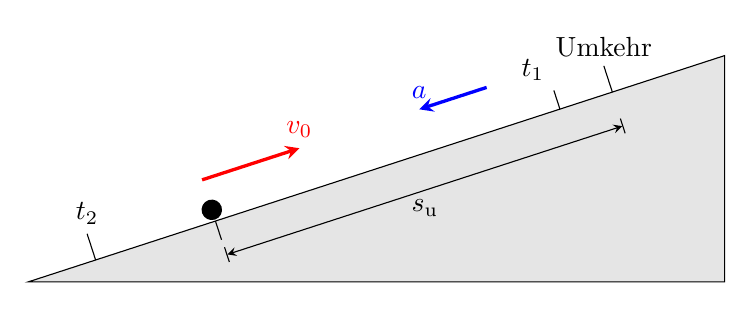
\begin{tikzpicture}[>=stealth]
 \fill[gray!20] (0,0) -- (8.844,0) -- (8.844,2.874) -- cycle;
 \draw (0,0) -- (8.844,0) -- (8.844,2.874) -- cycle;
 \begin{scope}[rotate=18]
  \fill (2.5,0.15) circle (0.13);
  \draw[->, very thick, red] (2.5,0.55) -- (3.8,0.55) node[above] {$v_0$};
  \draw[->, very thick, blue] (6.3,0.55) -- (5.4,0.55) node[above] {$a$};
  \draw (2.5,0) -- (2.5,-0.25);
  \draw (7.8,0) -- (7.8,0.35) node[above] {Umkehr};
  \draw (7.1,0) -- (7.1,0.25) node[above left] {$t_1$};
  \draw (0.9,0) -- (0.9,0.35) node[above] {$t_2$};
  \draw[|<->|] (2.5,-0.45) -- (7.8,-0.45) node[midway, below] {$s_\mathrm{u}$};
 \end{scope}
\end{tikzpicture}
\end{center}

Die Richtung den Hang hinauf ist positiv, der Startpunkt ist $s = 0$. Die Geschwindigkeit ist $v = v_0 + a\,t$, die Kugel kehrt um, wenn $v = 0$ ist, also nach
\begin{align}
 t_\mathrm{u} &= \tKuF = -\frac{\vKa}{\aK} = \tKu
\end{align}
Bis dahin ist die mittlere Geschwindigkeit $\frac{v_0+0}{2}$ und die Kugel rollt
\begin{align}
 s_\mathrm{u} &= \frac{v_0}{2}\,t_\mathrm{u} = \sKuF \\
   &= -\frac{\left(\vKa\right)^2}{2\cdot\left(\aK\right)} = \sKu \approx \result{\sKuP{0}{2}}
\end{align}
Da die Beschleunigung auch nach dem Umkehren gleich bleibt, gilt für den Ort zu jeder Zeit (mittlere Geschwindigkeit $\frac{v_0+v}{2}$ mal Zeit)
\begin{align}
 s &= \frac{v_0+\left(v_0+a\,t\right)}{2}\,t = v_0\,t+\frac{1}{2}a\,t^2
\end{align}
Nach $t_1 = \tKaO$ rollt die Kugel bereits wieder hinunter und ist
\begin{align}
 s_1 &= \sKaF \\
   &= \vKa\cdot\tKa+\frac{1}{2}\cdot\left(\aK\right)\cdot\left(\tKa\right)^2 = \sKa \approx \result{\sKaP{0}{2}}
\end{align}
vom Startpunkt entfernt (hangaufwärts). Nach $t_2 = \tKbO$ ist
\begin{align}
 s_2 &= \sKbF \\
   &= \vKa\cdot\tKb+\frac{1}{2}\cdot\left(\aK\right)\cdot\left(\tKb\right)^2 = \sKb
\end{align}
Die Kugel ist am Startpunkt vorbeigerollt (nach $2\,t_\mathrm{u}$) und befindet sich $\result{\sKbbP{0}{2}}$ unterhalb des Startpunkts, sofern die schiefe Ebene dort weitergeht.
